\documentclass[conference]{IEEEtran}
\usepackage{cite}
\usepackage{amsmath,amssymb,amsfonts}
\usepackage{algorithmic}
\usepackage{graphicx}
\usepackage{textcomp}
\usepackage{xcolor}
\usepackage{lineno,hyperref}

%% `Elsevier LaTeX' style
\bibliographystyle{IEEEtran}

\newcommand{\info}[1]{Department of Mechanical Engineering, University of S\~ao Paulo at S\~ao Carlos School of Engineering, S\~ao Carlos, Brazil. }
\newcommand{\email}[1]{email: #1}
\begin{document}
%\begin{frontmatter}
\title{Bipedal robot walking using reinforcement learning}

\author{
\begin{minipage}{0.40\textwidth}
	\centering
	Jhon Charaja \\
	\small{\textit{Department of Mechanical Engineering, University of S\~ao Paulo at S\~ao Carlos School of Engineering, S\~ao Carlos, Brazil.} } \\
	\email{jhon.charaja@usp.br}
\end{minipage}
\hfill
\begin{minipage}{0.40\textwidth}
	\centering
	Luca Borgonovi \\
	\small{\textit{Department of Mechanical Engineering, University of S\~ao Paulo at S\~ao Carlos School of Engineering, S\~ao Carlos, Brazil.} } \\
	\email{lucaborgonovi@usp.br}
\end{minipage}
}
	
\maketitle
\begin{abstract}
Mathematical models have been developed to describe the dynamic of bipedal walking activity. Some of these models are obtained with a simple physical interpretation of the system, and others consider a large number of nonlinear relationships and kinematic constraints to guarantee high precision and reliability. However, in some cases, using the more detailed models can be a challenging activity due to the number of parameters to be tuned. Likewise, it also does not guarantee the stability of dynamic system. For this reason, this work is focused on perform bipedal walking using a machine learning approach that does not require for a complex mathematical model or control formulation. On the one hand, the MuJoCo dynamic simulator is going to be used to simulate the dynamics of a two-legged robot. On the other hand, deep reinforced learning with the proximal policy optimization algorithm will be used for the robot to learn to walk.



% english version
%Clinical studies indicate that walking is an important activity for maintaining adequate levels of health, reducing the risk of chronic diseases, and performing day-to-day activities. For this reason, it is necessary to provide rapid physical rehabilitation to patients who have lost the ability to walk due to non-traumatic accidents. The main objective of this work is to indicate the range of motion of each joint to maintain balance during bipedal walking. In this way, it is expected to reduce the rehabilitation time of each patient by using this joint information and the appropriate rehabilitation exercises. On the one hand, the MuJoCo dynamic simulator is going to be used to simulate the dynamics of a two-legged robot based on the human frame. On the other hand, reinforced learning with the proximal policy optimization algorithm will be used for the robot to learn to walk. Finally, all the robot training will be analyzed to indicate how the joints were moved and activated to gain more stability. 
	
% spanish version
%Estudios clínicos indican que caminar es una actividad importante para mantener adecuados indices de salud, reducir el riesgo de enfermedades crónicas y realizar actividades del día a día. Por ese motivo, es importante brindar rápida rehabilitación física a los pacientes que han perdido la capacidad de caminar debido a accidentes no traumáticos. El objetivo de este trabajo es indicar cuales son las articulaciones más importantes para mantener el equilibrio durante la caminata bípeda. Por un lado, el simulador dinámico MuJoCo se va a usar para simular la dinámica del robot de dos piernas basado en la estructura humana. Por otro lado, aprendizaje reforzado con el algoritmo de proximal policy optimization se va a usar para que el robot aprenda a caminar. Finalmente, se va analizar todo el entrenamiento del robot para indicar como fue movimiento las articulaciones para ganar más estabilidad. De esta forma, se espera reducir el tiempo de rehabilitación de cada paciente usando esta información articular y los adecuados ejercicios de rehabilitación.	
\end{abstract}

\begin{IEEEkeywords}
	two-legged robot, reinforcement learning 
\end{IEEEkeywords}


\section{Introduction}
Mobile robots have gained more notoriety over the years, as the development of new technologies allows the implementation of these robotic systems in different areas: from agriculture to the exploration of satellites and planets \textbf{[reference]}. They are classified into wheeled, tracked, undulating, aerial and legged \textbf{[reference]}. In this way, they can use abilities already known in fixed robots (e.g. robotic manipulators), such as applying forces greater than those that a human being can perform with high precision, but with a mobile base. For this reason, they are able to perform repetitive, dangerous or demanding work that requires strength and precision, precision beyond what a human being is capable of, in distant places, without an individual needing to take the robot to the task site.

In this context, among the different types of mobile robots, perhaps the best known are wheeled robots due to the efforts to develop fully autonomous cars, and also because of rovers that currently explore Mars \textbf{[reference]}. However, using these robots in very rough terrain can bring some disadvantages, such as tipping due to some instability that the robot may have due to the unevenness of the ground. Factors that can interfere with the proper functioning of wheeled robots are, for example, holes, steps and steep slopes. In these cases, opting for legged robots is a good option, as they can get around these problems: legs can dodge holes, walk on steps and march up steep climbs.

The design of controllers that can keep these robots stable and functioning properly, becomes more difficult, since it is necessary to control numerous actuators, at the same time, in each of the legs, so that the robot can march correctly \textbf{[reference]}. Thus, there are different approaches to developing legged robot controllers\textbf{[reference]}. Some of them involve the use of previous robot information, such as dynamic models and computer simulations. However, it is not always so easy to obtain this data, which can complicate the design of the controller. Other approaches involve the use of machine learning, eliminating the need to model the dynamic behavior of the robot, as it will learn from its own mistakes \cite{kormushev2013reinforcement}.

Deep reinforcement learning (DRL) is a machine training method to teach an agent to take a good sequence of decisions (actions) \cite{sutton2018reinforcement}. DRL works with the simple idea of giving positive (reward) or negative (punishment) reinforcement to the agent's behavior. In this way, the agent learns to make decisions that guarantee the highest amount of reward. Due to its simple operating mechanism, DRL can be adapted to solve complex optimization problems in the robotics area \cite{kober2013reinforcement}. For this reason, recent works use DRL with proximal policy optimization (PPO) algorithm to control the waking of Cassie, ABL-BI and Robotis-op3 robots \cite{xie2018feedback}, \cite{beranek2021behavior}, \cite{jiang2020motion}. In these three works, the agent learned strategies to maintain the body's balance despite external disturbances of force and uneven terrain. 

Currently, there are several methods to develop drivers for robots with legs. The classic ones use previous knowledge about the robot, such as its dynamic model or information obtained from simulations involving them. For example, the ANYmal robot from ETH uses the inverted pendulum model to generate joint torques, contact forces and motion \cite{anymal}; the MIT Cheetah uses a model predictive control to plan desired contact forces \cite{cheetah}.

However, in certain cases, it can be difficult to obtain prior knowledge of the robot through dynamic models and simulations. In this context, a feasible approach to controller design is to use deep learning, more specifically, deep reinforcement learning. Furthermore, another advantage that the use of machine learning provides is that it does not accumulate data generated by the robot, it only uses what is currently being processed, in addition to the fact that the robot can learn to march on its own \cite{haarnoja2018learning}.

Controller development methods using deep reinforcement learning may vary depending on the chosen algorithm. The University of California, for example, used a learning algorithm based on maximum entropy reinforcement learning, training a Minitaur robot directly, without having to train a simulation beforehand \cite{haarnoja2018learning}.

The proximal policy optimization algorithm formulate a objective function related with the reward and then use the gradient of the objective function to seek the optimal policy \cite{schulman2017proximal}. PPO is one of the best algorithms for reinforcement learning applications due to its simplicity and high efficiency~\cite{schulman2017proximal}. This algorithm has been successfully implemented to solve problems in bipedal walking \cite{melo2019learning}, games \cite{kristensen2020strategies} and unmanned aerial vehicles \cite{bohn2019deep}.


This work perform the walking of a bipedal robot using deep reinforcement learning with proximal policy optimization. For this purpose, the MuJoCo simulator is used to compute the dynamics of the bipedal robot. Likewise, OpenAI gym toolkit is used to compute the reinforcement learning equations.

% first draft
The document is structured as follows. First, section II explain reinforcement learning method. Second, section III describes the policy proximal optimization algorithm. Third, section IV indicates the open-source libraries and simulator used in this work. Section V presents the results of the work. Finally, section VI describes conclusions 



\graphicspath{{images/methodology/}}
\section{Reinforcement learning}
The reinforcement learning method trains an agent to take the optimal sequence of decisions \cite{sutton2018reinforcement}. The learning process uses positive and negative reinforcement to increase or decrease the probability of choosing an specific action. In this sense, the agent learns, through an iterative process, to make the sequence of decisions that maximizes the amount of reward that he will receive \cite{sutton2018reinforcement}.

\begin{figure}[h!]
	\centering
	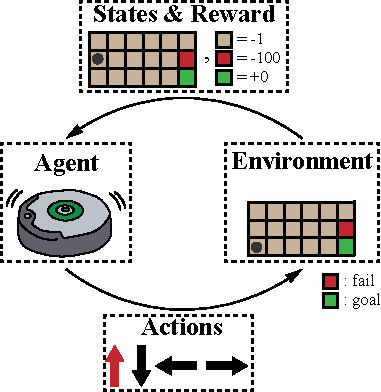
\includegraphics{reinforcement_learning_diagram.pdf}
	\caption{Reinforced learning framework for the application that a mobile robot must reach the desired position. In this example, the agent's actions are up, down, right and left; likewise, the agent's objective is reach the green cell and the agent fails when reach the red cell.}
	\label{fig:RL_framework}
\end{figure}

The framework of reinforcement learning is formed by four elements: (i) agent, (ii) actions, (iii) environment, and (iv) states and rewards \cite{sutton2018reinforcement}. Figure \ref{fig:RL_framework} describes the reinforcement learning framework for the application that a mobile robot must reach the desired position. First, an agent is the entity who takes decisions based on the reward and punishment that he will receive. Second, action space are all the available actions that the agent could use to interact with the environment. Third, the environment is the space where the agent lives and interact. Fourth,  the new agent's state after applying an action in the environment and the reward associated with that specific action. This process will be repeated several times until the agent learns a successful strategy to interact with the environment and maximize the reward.

In reinforcement learning, the agent's strategy is called policy ($\pi(s|a)$) and indicates which actions the agent should chooses in each state \cite{sutton2018reinforcement}. Policies are usually stochastic to consider the uncertainties and probabilities of real world \cite{tedrake2004stochastic}.  In this way, policies assign a probability of success to each action, and the agent chooses the action with the highest probability. Hence, the objective of reinforcement learning algorithms is to find the optimal policy that maximizes the amount of reward. 

The sum of the accumulated rewards from an initial state $s_t$ is the standard way of quantifying how good or bad the policy is \cite{sutton2018reinforcement}. This quality parameter is called value function ($V^{\pi}(s_t)$) and indicates the discounted sum of rewards that an agent will obtain starting in state $s_t$ and following the policy $\pi$ \cite{sutton2018reinforcement}. The value function can be computed as
\begin{equation*}
	V^{\pi}(s_t= s) = E_{\pi}  \left[r_t + \gamma r_{t+1} + \gamma^{2} r_{t+2}+ . . . | s_t = s \right],
\end{equation*}
\noindent where $r_t$ is the reward at time $t$, $\gamma$ is a discounted term and $s_t$ is the initial agent's state. However, calculating the value function requires the agent to start in all available states of the environment and in complex activities this can require a large amount of storage and computational cost. For this reason, more recent work uses deep neural networks to estimate the value function and optimal policy \cite{henderson2018deep}.

\begin{figure*}[t]
	\centering
	\subfloat[]{\includegraphics{policy_cnn.pdf}}
	\hfill
	\subfloat[]{\includegraphics{value_function_cnn.pdf}}
	\caption{Deep neural networks scheme: (a) predict optimal action and (b) estimate value function.}
	\label{fig:rl_cnn}
\end{figure*}

\section{Deep reinforcement learning}
Deep reinforcement learning (DRL) represent the combination of deep neural networks with reinforcement learning framework \cite{li2017deep}. Deep neural networks estimate the value function and predict the policy actions considering the agent's state as input. Figure \ref{fig:rl_cnn} describes the policy and value function parameterized with a neural network. Therefore, the goal of DRL is to find the neural network parameters that describe the optimal policy that generates the highest reward.

The policy gradient method optimizes the parameters of a neural network that define the behavior of the policy, and in this way, maximize the accumulated reward \cite{sutton2018reinforcement}. The policy gradient algorithms formulate an objective function related to the accumulated reward and then use the gradient ascent method to modify the parameters of the neural network~\cite{thomas2017policy}. The general form of the objective functions of the policy gradient algorithms is given by
\begin{equation*}
	L(\theta) = \expectation \left[ \mathrm{log} \pi_\theta (a|s) \advantage  \right],			
\end{equation*}
with,
\begin{equation*}
	\advantage = V^{\pi_{\theta}}_{t}  - \hat{V}_{t}, 
\end{equation*}
\noindent where $L(\theta)$ is the objective function, $\pi_\theta (a|s)$ is policy parameterized with neural network parameters ($\theta$), $\advantage$ is advantage function, $V^{\pi_{\theta}}_{t}$ is accumulated reward following policy $(\pi_\theta)$ and $\hat{V}_{t}$ is expected accumulated reward by the neural network.


\section{Proximal policy optimization}
PPO is a recent policy gradient method that strikes a good balance between rapid implementation and efficiency \cite{schulman2017proximal}. The PPO algorithm seeks to maximize accumulated reward, minimize estimation error of value function and explore different sequence of actions. Likewise, the PPO algorithm adds upper and lower limits to avoid large modifications of the neural network parameters \cite{schulman2017proximal}. In this way, PPO increases stability and reduces oscillations during neural network training.

The main objective function of PPO algorithm is given by
\begin{equation*}
	L^{\mathrm{CLIP}}(\theta) = \expectation \left[ \mathrm{min} \left(  r_{t}(\theta)  \advantage,  \mathrm{clip} (r_{t}(\theta) , 1-\epsilon, 1+\epsilon) \advantage  \right)  \right],	
\end{equation*}
with,
\begin{equation*}
	r_{t}(\theta) =\ratio,			
\end{equation*}
\noindent where $r_{t}(\theta)$ is the probability ratio between new and old policies, $\mathrm{clip}(\cdot)$ is the clip function to limit upper and lower increments, and $\epsilon$ is an hyperparameter that usually is  $0.2$ \cite{schulman2017proximal}.


The complete objective function of PPO algorithm can be computed as
\begin{equation*}
	L^{\mathrm{PPO}}(\theta) = \expectation \left[  L^{\mathrm{CLIP}}(\theta) - c_1 L^{\mathrm{VF}}(\theta)  + c_2 S[\pi_\theta](s_t)  \right],			
\end{equation*}	
with,
\begin{equation*}
	L^{\mathrm{VF}}(\theta) = \left( V_\theta (s_t) - V^{\mathrm{target}}_{t}  \right)^{2},	
\end{equation*}			
\noindent where $L^{\mathrm{CLIP}}(\theta)$ is the main objective function, $c_{1,2}$ are hyperparameters, $L^{\mathrm{VF}}(\theta)$ is square-error loss and $S$ is an entropy term to increase exploration \cite{schulman2017proximal}.

\section{Experimental setup}

\subsection{Bipedal robot simulation}
The legged robot has two legs (right and left). Likewise, each leg has three joints (ankle, knee, hip) and one joint for trunk orientation. Therefore, the robot has $14$ states considering position and velocity. Finally, the dynamic behavior of the bipedal robot is computed with the Multi-Joint dynamics with Contact (MuJoCo) physics simulator \cite{todorov2012mujoco}. Figure \ref{fig:bipedal_robot} describe the bipedal robot in a simulation environment of MuJoCo simulator.

\begin{figure}
	\centering
	\includegraphics{bipedal_robot.pdf}
	\caption{Bipedal robot in MuJoCo simulator. In this simulation environment, the robot has a trunk, left and right legs. Likewise, three joints in each leg (ankle, knee and hip).}
	\label{fig:bipedal_robot}
\end{figure}	

\subsection{Reinforcement learning: reward configuration}
The algorithm must learn to balance the robot as it moves forward. In this sense, the algorithm must receive positive reward based on the time that it maintains the balance when walking. Hence a simple way to set up the reward system is to give positive reward until the robot loses its balance. On the one hand, we establish that the robot loses its balance when the trunk's angular position is greater than $50^{\circ}$. On the other hand, the robot receives a positive reward of +1 for each iteration that maintains balance and a reward equal to the magnitude of the linear speed of the whole body to encourage forward movement.

\section{Methodology}

\subsection{Deep Reinforcement Learning: Policy Gradient Method}

\subsection{Simulation Environment and Libraries}

The Policy Gradient algorithm was implemented in Python language using the TensorFlow library, which is an open-source library for artificial intelligence and machine learning.

To carry out the simulations, the MuJoCo software was used (Multi-Joint Dynamics with Contact), a simulator for multi-body dynamics with contact. The computational model used to implement the algorithm was a two-dimensional bipedal robot Walker2d-v2, which has 7 joints and two translational movements (horizontal and vertical). During the simulation, the model went through 40 million states to assess how gait evolved as the Policy Gradient algorithm was implemented.

All simulations were carried out on a computer with Intel\textregistered Core\texttrademark i7-8750H 2.20 GHz processor, 8.00 GB of RAM, 128 MB dedicated video card, Windows 10 Home Single Language 64 bits. The Python version XXX and the MuJoCo XXX were the platforms where the simulations took place.
\section{Results}
The model receives a reward ($+1$) every second that trunk lean is less than $30^{\circ}$. Figure \ref{fig:boxplot} shows variation of reward with respect to number of training iterations for $10$, $20$, $30$ and $40$ million. In this figure, red line indicates mean value, horizontal lines maximum and minimum values. Likewise, the reward that model gets with $20$ million is greater than with $10$ million. This is because the model learns to walk better with more training time. However, the reward that model gets with $30$ and $40$ million is less than with $20$ million. This is because model is trying/learning to use both legs instead of just one\footnote{visual material of the training of the two-legged robot in \url{https://www.youtube.com/watch?v=Vt20_SWR2xI&ab_channel=LucaBorgonovi}}.


\begin{figure}
	\centering
	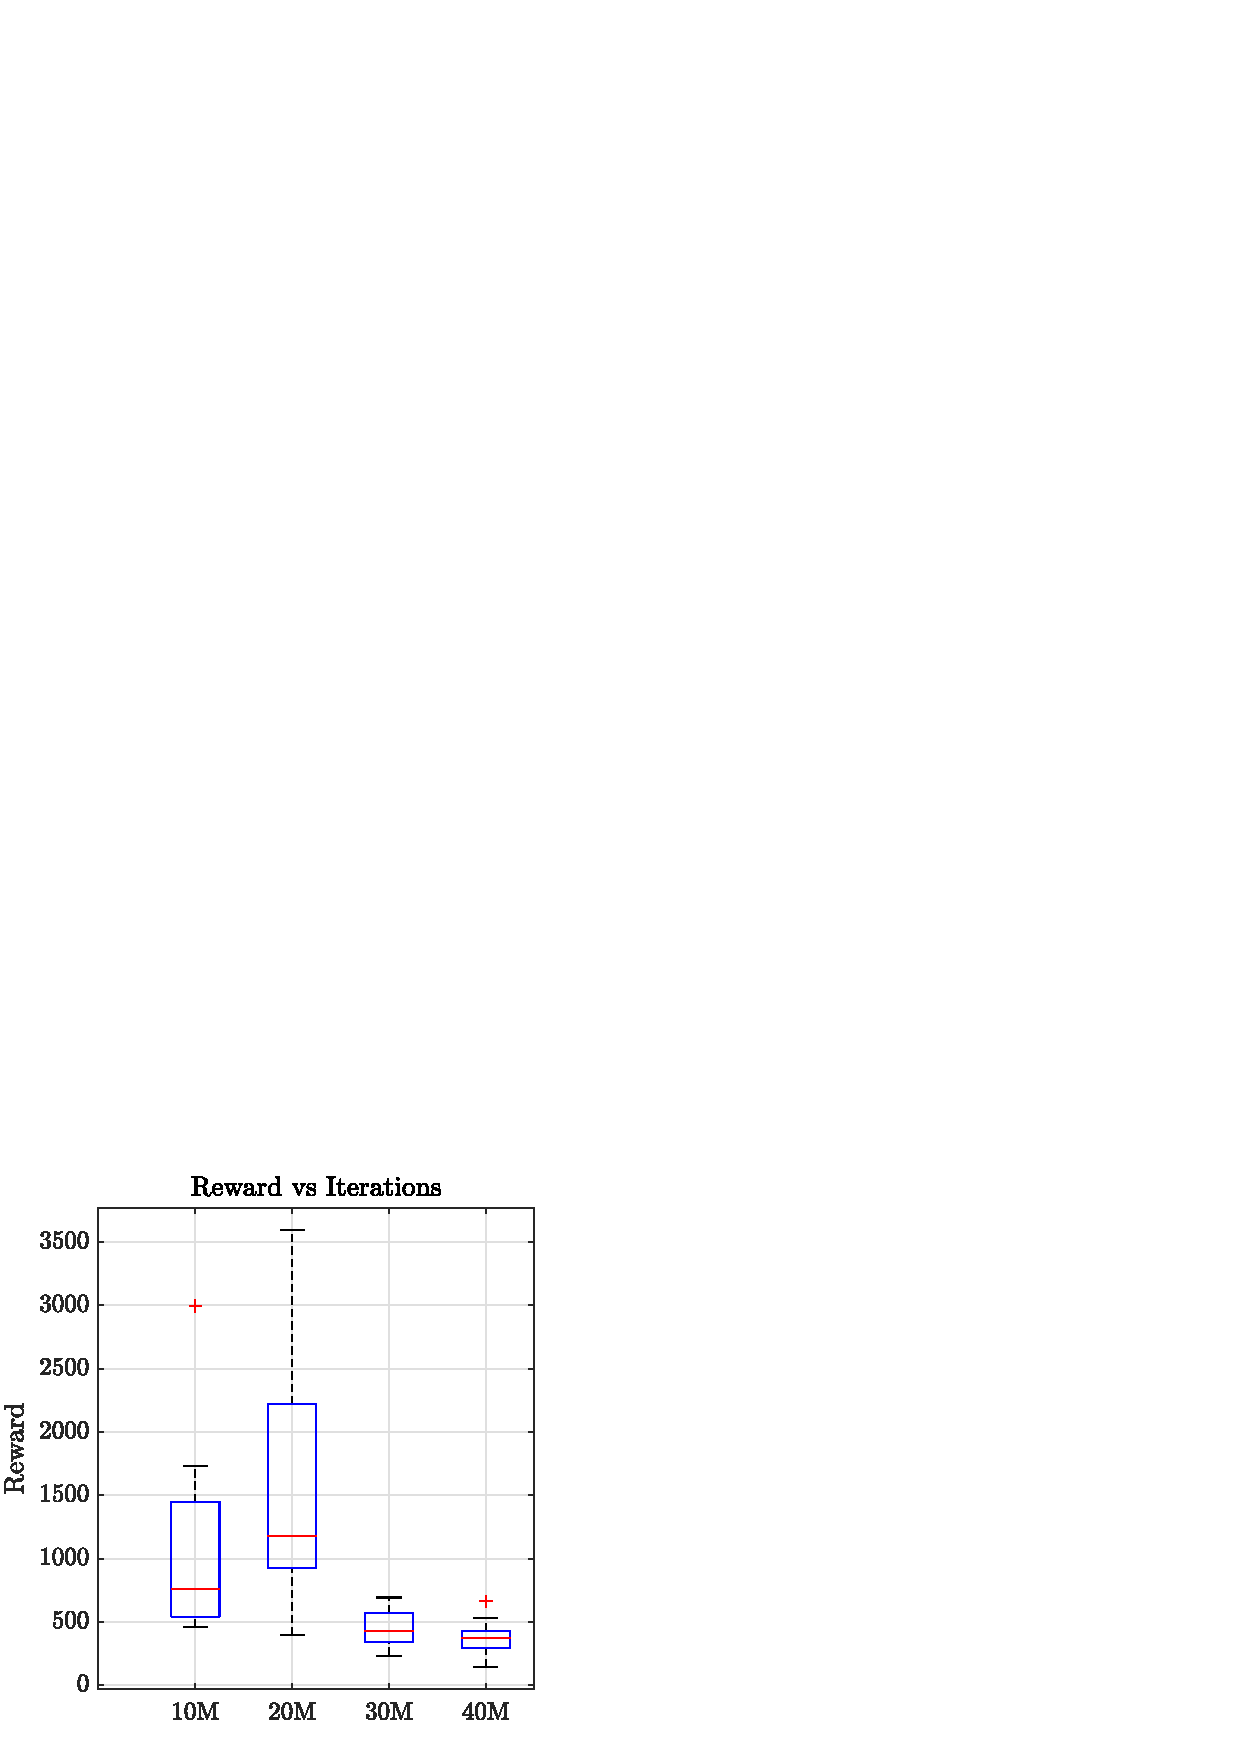
\includegraphics{images/reward_vs_iter.pdf}
	\caption{Performance of trained model to keep the trunk lean below $30^{\circ}$.}
	\label{fig:boxplot}
\end{figure}




% bibliography
\bibliography{mybibfile}

	
\end{document}